% Chapter Template

\chapter{Extensions to the Wages and Tait trial design} % Main chapter title

\label{WT} % For referencing this chapter elsewhere, use \ref{WT}

%----------------------------------------------------------------------------------------
%	SECTION 1
%----------------------------------------------------------------------------------------

%\section{Plan for this Chapter}

%The main plan for this chapter will be as follows. It will comprise of three sections an Introduction / background then two section on the each of the Wages and Tait modifications. One for the randomisation and one for the time-to-event component. 

%-----------------------------------
%	SUBSECTION 1
%-----------------------------------
%\subsection{Introduction Plan}

%I say Introduction but this can most likely be split into 2 sections. It can serve as an introduction to Phase I/II trials and an introduction to Wages and Tait specifically, which will include the maths. 

%\begin{enumerate}
%	\item A background on adaptive phase I/II designs - mainly a motivation / rationale for why they are used.
%	\item Some examples of these types of designs obviously can use efftox and wages and tait here. Can look at Kristian's PhD here as he has some examples. It may also be worthwhile to do a literature review to look into other designs. 
%	\item Include a paragraph stating aims of the chapter or whats included.
%	\item Include further details on wages and tait which will then lead to the specific maths for an un modified design.
%\end{enumerate}


%-----------------------------------
%	SUBSECTION 2
%-----------------------------------

%\subsection{Randomisation Modification Plan}
%Not sure what this section should be called. Perhaps something along the lines of Randomisation to control modification. 

%\begin{enumerate}
%	\item Start off with rational, why we would want to include randomisation to control 
%	\item Point out that this could already be done by including a dose as control. However, point out that it is unlikely to recruit or more so you can't guarantee that patients will be allocated that dose as it will be relatively low on efficacy in the AR phase. This is the main distinction with this modification we fix some randomisation. 
%	\item Go into the maths. Should only be a small modification in the adaptive randomisation phase. 
%	\item Simulations. Need to present a basic design then contrast it something. A quick idea is to have the same trial but then change the percentage that are allocated to placebo. Then contrast this with a trial that does randomisation AT recruitment i.e. 2:1 then enter Wages and Tait. So compare 2:1 to a 33\% fixed, 3:1 to 25\%, 4:1 to a 20\% etc ... Should be easy to make some plots for this. Can also investigate the impact of altering the number of patients in the adaptive randomisation phase, like I did for those quick simulations where I had it set at 26 then 52. 
%	\item Observations from running SPIN-SCI simulations. Running a shortened adaptive randomisation phase and front-loading patients onto control seems to result in better operating characteristics when compared to a standard Wages and Tait design. Another comparison to look at hear would be a wages and tait design with a further reduced adaptive randomisation phase. One point to make could be that this front loading could be used in normal wages and tait designs where you want to be extra careful with recruitment and for safety reasons want to fix recruitment at the lowest dose-level before escalating. 
%\end{enumerate}


%-----------------------------------
%	SUBSECTION 3
%-----------------------------------

%\subsection{Time-to-event Modification Plan}
%This should be more straight forward. Will probably have to work more on the code for this one. 

%\begin{enumerate}
%	\item Again start with rational for why this modification might be useful. Can elude to some stuff mentioned in the Adept chapter. 
%	\item How this impacts the maths what equations are altered etc. 
%	\item Simulations. Consider a simple trial with a long follow-up period and then simulate using normal wages and tait and then the TITE modification. Can look at the original TITE paper to look how they made comparisons between the designs. May be beneficial to track things like duration also. 
%\end{enumerate}


%----------------------------------------------------------------------------------------
%	SECTION 1
%----------------------------------------------------------------------------------------

\section{Introduction}
\label{WT:Introduction}

Typically the main aim of Phase \RN{1} clinical trials is to identify the maximum tolerated dose (MTD) of the treatment being investigated. The MTD is usually determined under the cytotoxic assumption which assumes the most toxic dose is the most efficacious. With model based designs such as the continual reassessment method (CRM) \cite{oquigleyContinualReassessmentMethod1990} escalation occurs to identify the dose with an associated probability of toxicity based on a pre-defined target. Dose selection and escalation decisions do not consider efficacy rather they are determined based on the occurrence of toxicities. The cytotoxic assumption here implies that rate of efficacy increases monotonically with the probability of toxicity and dose level. Subsequent Phase \RN{2} trials aim to assess the efficacy of the treatment at the recommended dose (MTD). Usually these two phases are conducted independently of each other and as such the ability to share information across the phases is somewhat lost. 

For treatments like chemotherapy which kills all cells including cancer cells the cytotoxic assumption is valid. However, the emergence of modern treatments such as immunotherapy and molecular targeted agents challenges this paradigm. Immunotherapy is a form of treatment which utilises the body's own immune system to fight the cancer. Molecular targeted agents work by interfering with specific molecules responsible for the growth, spread and progression of cancer. The monotonic assumption of dose-toxicity and dose-efficacy may not hold for these new types of treatments. Furthermore, these treatments in general are less toxic than traditional cytotoxic agents such as chemotherapy therefore it is possible the most efficacious dose may occur at a dose level below the MTD \cite{ahnOptimalBiologicalDose2016}. This produces some methodological challenges for dose-finding trials. Instead of trying to identify the MTD the goal would be to determine the optimal biological dose (OBD). Depending on the aims of the trial and the design implemented the definition of the OBD may vary. The OBD could be a dose that provides the maximum probability of efficacy with the probability of toxicity being less than a pre-defined target value, or the dose that has a beneficial trade-off between toxicity and efficacy. In order to determine an optimal dose both toxicity and efficacy outcomes need to be considered, this leads to a need for joint phase \RN{1}/\RN{2} trial designs. Here we will briefly explore some of these designs. 

Braun \cite{braunBivariateContinualReassessment2002} proposed the bivariate continual reassessment method (bCRM), an extension to the CRM which incorporates competing outcomes for both toxicity and disease progression. The design models the probabilities of toxicity and progression independently, it is suggested that either empiric, logistic and hyperbolic tangent functions are used dependent on their biological plausibility. Both outcomes are then combined into a joint distribution which is used to estimate posterior means based on priors and observed data. 

Thall \& Cook \cite{thallDosefindingBasedEfficacytoxicity2004} developed EffTox , a Bayesian adaptive dose-finding trial based on trade-offs between the probabilities of toxicity and efficacy. Marginal probabilities of efficacy and toxicity at each dose are modelled and used with utility contours to determine the desirability of each dose based on posterior probabilities of efficacy and toxicity \cite{brockImplementingEffToxDosefinding2017}. 

Zhou et al. \cite{zhouUtilitybasedBayesianOptimal2019} introduced a Utility-based Bayesian Optimal Interval (U-BOIN) phase \RN{1}/\RN{2} design to identify the OBD. This design is an extension of the Bayesian optimal interval (BOIN) design for phase \RN{1} trials developed by Liu and Yuan \cite{liuBAYESIANDATAAUGMENTATION2013}. U-BOIN jointly models toxicity and efficacy with a multinomial-Dirichlet model and uses a utility function to measure the dose risk-benefit trade-off. The design consists of two seamless stages. Firstly, in stage \RN{1} the BOIN design is used to explore the dose levels and determine a set of admissible doses and collect preliminary efficacy data. In stage \RN{2} posterior estimates of utility for each dose are continuously updated after each cohort this is done using toxicity and efficacy data from both stages. 

Zhang et al. \cite{zhangAdaptiveDosefindingDesign2006} introduced the trivariate CRM (TriCRM) design. The design considers patients to have one of three possible outcomes: no efficacy and toxicity, efficacy without toxicity and toxicity. These outcomes are then modelled using a continuation-ratio model. A Bayesian approach and dose-finding algorithm is then used to identify the OBD similar to the CRM.  

Anathakrishnan et al. \cite{ananthakrishnanExtensionsMTPITEQR2018} produced extensions to the modified Toxicity Probability Interval (mTPI) design by Ji \& Wang \cite{jiModifiedToxicityProbability2013} and Toxicity Equivalent Range (TEQR) design by Blanchard \& Longmate \cite{blanchardToxicityEquivalenceRange2011} to include efficacy outcomes. In both designs isotonic regression is applied to the observed DLT rates at the end of the trial. Dependent on the shapes of the dose-response curves and the underlying response rates isotonic regression is applied on the observed response rates or the differences in observed response rates to determine the optimal dose. 

Riviere et al. \cite{rivierePhaseIIDosefinding2018} developed a Bayesian dose-finding design for MTA. The design works on the premise that for MTA efficacy initialy increases with dose then eventually plateaus. They use a logistic model with a plateau parameter to capture the dose-level at which plateaus begin in  the dose-efficacy relationship. A weighted likelihood approach is also used to accommodate for any potential late-onset toxicities. This methodology incorporates adaptive randomisation to allocate dose-levels close to the likely plateau point.

This chapter revolves around the seamless phase \RN{1}/\RN{2} dose-finding adaptive design by Wages and Tait \cite{wagesSeamlessPhaseII2015}, that we will refer to as the WT design. This design models toxicity and efficacy independently. To model the probability of efficacy a set of possible efficacy skeletons are considered which would correspond to plausible dose-efficacy relationships. For the class of dose-efficacy models a single parameter model is used similar to the empiric model of the CRM. The authors recommend that ($2n - 1$) efficacy skeletons are specified where $n$ is the number of doses being investigated. Toxicity is modelled using a CRM approach with an empiric model. As such a skeleton for toxicity is also required for this design. The dose-finding operates in two stages the adaptive randomisation (AR) phase and the maximisation phase. In the AR phase patients are adaptively randomised amongst a set of tolerable doses, where probabilities of randomisation to each dose are proportional to their posterior probabilities of efficacy. A pre-defined number of patients enter the AR phase and once recruitment has completed we move to the maximisation phase. In this phase patients are allocated to the dose in the tolerable set which maximises probability of efficacy.  

The incorporation of an AR phase early on into the trial is beneficial since there may be a lack of data in order to rely on decisions made by the maximisation of efficacy probabilities. Also there may be doses that haven't been tested and randomisation allows for information to be collected from these. It also helps avoid getting stuck repeatedly recruiting to the same dose and allows for a more broad understanding of the dose-efficacy and toxicity relationships. One extension we propose is the inclusion of randomisation to a control arm into the design. This would provide a set of patients who receive standard of care to act as controls and allow for comparisons to be made with outcomes from patients receiving the OBD. There is also the added benefit of being able to include standard of care into the models to get a better understanding of the dose-efficacy and toxicity relationships.  

In Section \ref{WT:Wages-and-Tait-Design}, details the statistical aspects of the WT design and how it works. We introduce our extension to the design to include randomisation to control in Section \ref{WT:RtC-WT}. Section \ref{WT:Evaluation-of-the-Extension} evaluates the performance of the new design with a simulation study. Finally, discussions and conclusions are presented in Sections \ref{WT:Discussion} and \ref{WT:Conclusion} respectively.  


%----------------------------------------------------------------------------------------
%	SECTION 2
%----------------------------------------------------------------------------------------
\section{The Wages and Tait Design}
\label{WT:Wages-and-Tait-Design}

In this section we detail the Wages and Tait design following the introduction of some notation. A set of $I$ doses under investigation can be denoted as $\mathscrsfs{D} = \{d_1, ...,d_i\}$. For each patient $j$ entered into the trial they are allocated to a dose level and joint outcomes for toxicity and efficacy are measured. The dose for the $j$th patient, $X_j$, $j = 1,...n$ can be thought of as random, taking values $x_j \in  \mathscrsfs{D}$. Let $Y_j$ and $Z_j$ be the random variables for binary toxicity and efficacy events respectively. For an individual patient $j$ toxicity and efficacy outcomes can take values $y_j, z_j \in \{0,1\}$ where 0 indicates and event didn't happen and 1 indicates that it did. 

Wages and Tait \cite{wagesSeamlessPhaseII2015} utilise the CRM approach of O'Quigley et al. \cite{oquigleyContinualReassessmentMethod1990} to model toxicity. A univariate Bayesian method is used which begins by assuming a monotonically increasing dose-toxicity curve. The DLT probabilities, $\pi_T(d_i)$, are modelled at each dose level $i$ where $i= 1, ..., I$. The power model is specifically used by Wages and Tait in this design given by 

\begin{equation}
\label{WT:eq_power-model}
F(d_i, \beta) = p_i^{exp(\beta)}
\end{equation}

A working model or skeleton containing the prior beliefs of toxicity at each dose level are provided by investigators in the form $0 < p_1 < ... <p_I <1$. For the single parameter in the power model $\beta$ we assume it has a prior distribution $g(\beta)$. After the inclusion of $j$ subjects into the trial, we have  data in the form of $\Omega_j = \{(x_1,y_1,z_1), ..., (x_j,y_j,z_j)\}$. The toxicity data can be used with Equation \ref{WT:eq_power-model} to give the likelihood for $\beta$

\begin{equation}
L(\beta|\Omega_j)=\prod_{l=1}^{j}\{F(x_l,\beta)\}^{y_l}\{1-F(x_l,\beta)\}^{1-y_l}  
\end{equation}

the posterior density for $\beta$ can be calculated using  

\begin{equation}
P(\beta|\Omega_j) = \frac{L(\beta|\Omega_j)g(\beta)}{\int_{-\infty}^{\infty}L(\beta|\Omega_j)g(\beta)d\beta}. 
\end{equation}

This can then be use to establish the posterior mean of $\beta$

\begin{equation}
\hat{\beta}_j = \int_{-\infty}^{\infty}\beta P(\beta|\Omega_j)d\beta
\end{equation} 

Using $\hat{\beta}_j$ estimates of DLT probabilities at each dose level can be obtained via 

\begin{equation}
\hat{\pi}_T(d_i) = F(d_i, \hat{\beta}_j) = p_i^{exp(\hat{\beta}_j)}. 
\end{equation}

For a specific maximum acceptable toxicity rate $\phi_T$ a set of acceptable or admissible doses can be declared as follows

\begin{equation}
\mathscrsfs{A}_j = \{d_i : \hat{\pi}_T(d_i)  \leq \phi_T ; i = 1,...,I \}.
\end{equation} 

To model efficacy a Bayesian approach is taken similar to how toxicity was modelled but rather than using a singular working model a class of working models are considered. They use a class of skeletons which correspond to various dose-efficacy relationships. These relationships might be monotonically increasing (as dose increases efficacy increases), unimodal (initially increasing then decreasing) or plateau (initially increase then level off). As a guide it is suggested that $(2I-1)$ working models should be specified. The probability of an efficacious response at dose $d_i$ is denoted as $\pi_E(d_i)$. The primary aim of the trial is to identify the optimal dose $d_v \in \mathscrsfs{D}$ which is defined such  that 

\begin{equation}
\pi_E(d_1) \leq ... \leq \pi_E(d_v) \geq ... \geq \pi_E(d_I). 
\end{equation}

Let $K$ denote the number of efficacy skeletons being used. Then for each skeleton $k$ we have $0 < q_{1k} < ... <q_{Ik} <1$ and for a particular skeleton $k; k = 1,...,K$ the true probability of efficacious response $\pi_E(d_i)$ at $d_i$ is modelled by 

\begin{equation}
\pi_E(d_i) = Pr(Z_j = 1|d_i) \approx G_k(d_i,\theta) = q_{ik} ^{exp(\theta)}
\end{equation}

As with the modelling of toxicity the power model is used again. Similarly as with $\beta$ a prior distribution $h(\theta)$ is assumed for $\theta$. For both the toxicity and efficacy models a Normal prior is used as first suggested by O'Quigley and Shen \cite{oquigleyContinualReassessmentMethod1996} such that $\beta, \theta \sim N(0,1.34)$. Additionally for the modelling of efficacy prior information regarding the plausibility of each model is taken into account using a weight function $\upsilon(k) = \{\upsilon(1), ..., \upsilon(K)\}$, where $\upsilon(k) \geq 0$ and where $\sum_k \upsilon(k) = 1$. If no information is available a discrete uniform distribution can be specified for $\upsilon(k)$. After $j$ patients have been included and observed in the study we have efficacy data from $\Omega_j$ and the likelihood model under $k$ is given by 

\begin{equation}
L(\theta|\Omega_j)=\prod_{l=1}^{j}\{G_k(x_l,\theta)\}^{z_l}\{1-G_k(x_l,\theta)\}^{1-z_l}  
\end{equation}

the posterior density is 

\begin{equation}
P(\theta|\Omega_j) = \frac{L(\theta|\Omega_j)h(\theta)}{\int_{-\infty}^{\infty}L(\theta|\Omega_j)h(\theta)d\theta}
\end{equation}

and under skeleton $k$ the posterior mean is given by 

\begin{equation}
\hat{\theta}_{jk} = \int_{-\infty}^{\infty}\theta P(\theta|\Omega_j)d\theta.
\end{equation} 

This information can be used to establish posterior model probabilities 

\begin{equation}
w(k|\Omega_j) = \frac{\upsilon(k)\int_{-\infty}^{\infty}L_k(\theta|\Omega_j)h(\theta)d\theta}{\sum_{k=1}^{K}\upsilon(k)\int_{-\infty}^{\infty}L_k(\theta|\Omega_j)h(\theta)d\theta}
\end{equation}

The posterior model probabilities are then used to determine which skeleton will be selected to model the dose-efficacy relationship. Each time a new patient is to be entered into the study and a dose-escalation decision needs to be a made, the skeleton $k^*$ with the largest posterior probability is selected such that

\begin{equation}
k^* = arg \; \underset{k}{max}w(k|\Omega_j).
\end{equation}

After determining the best skeleton and calculating the posterior mean of $\theta$ estimates of efficacy probabilities are then generated for each dose. 
\begin{equation}
\hat{\pi}_E(d_i) = G_{k^*} (d_i, \hat{\theta}_{jk^*})
\end{equation}

Dose-finding is conducted in two stages. The first stage begins with the adaptive randomisation (AR) phase. Here the next dose is randomly selected from the set of admissible doses. Randomisation probabilities for each dose are proportional to $\hat{\pi}_E(d_i)$ so that doses with higher estimated efficacy are more likely to be assigned to patients. For doses in $\mathscrsfs{A}_j$ their adaptive randomisation probability $R_i$ is 

\begin{equation}
\label{WT:eq_WT-ARprob}
R_i = \frac{\hat{\pi}_E(d_i)}{\sum_{d_i \in \mathscrsfs{A}_j}\hat{\pi}_E(d_i)}. 
\end{equation}

The AR phase lasts for a subset of $j_R$ patients such that $j_R \leq J$, where $J$ is the total number of patients to be entered into the trial. Wages and Tait suggest as a general rule of thumb to allocate 50\% of patients to both stages. It was shown that this approach works well in a variety of scenarios. However, this can be easily be adapted to suit individual trials. 

Once the AR phase has been completed the design switches to the second stage called the maximisation phase. Here the next dose is the dose from the admissible set with the highest estimated probability of efficacy. For a dose-escalation decision that needs to be made in the maximisation phase for the $(j+1)$th patient the dose $x_{j+1}$ is selected from the admissible set of doses $\mathscrsfs{A}_j$ with the highest estimated efficacy probability $\hat{\pi}_E(d_i)$ i.e. 

\begin{equation}
x_{j+1} = arg \; \underset{d_i \in \mathscrsfs{A}_j}{max}\hat{\pi}_E(d_i)
\end{equation}

The design also incorporates stopping rules for safety and futility. The safety rule stops the trial if too much toxicity is observed at the lowest dose level. This rule is applied throughout the trial for each dose-escalation decision. Exact binomial 95\% confidence intervals are calculated for the lowest dose. The lower bound of the interval is then compared to the acceptable toxicity rate $\phi_T$. If the lower bound interval is greater than the acceptable rate it can be said that the treatment is too toxic to warrant further investigation. Patients need to have been observed at the lowest dose in order for this rule to trigger, if there is no data available at the lowest dose the binomial confidence interval is effectively 0. 

The futility rule stops the trial if there are too few observed efficacy events. This rule only comes into play during the maximisation phase. This rule uses a similar method to the stopping rule by utilising binomial 95\% confidence intervals. During the maximisation phase the dose with the highest probability of efficacy is selected. At this point the 95\% binomial confidence interval is calculated for the current dose and if the upper bound is less than the futility threshold $\phi_E$ the trial is stopped as the treatment is inefficacious at all doses. Although 95\% confidence intervals are used by Wages and Tait these can be altered accordingly. 


 %----------------------------------------------------------------------------------------
 %	SECTION 3
 %----------------------------------------------------------------------------------------
 \section{RtC-WT: An extension to the Wages and Tait Design}
 \label{WT:RtC-WT}
 
 In this section we introduce our proposed extension to the Wages and Tait (WT) design named Randomisation to Control Wages and Tait (RtC-WT). As the name states, the design will allow investigators to utilise the WT design with the ability to recruit patients to a control arm. This idea was initially conceived by Kristian Brock (KB) whilst working on the design of a new dose-finding trial.  
 
 %-----------------------------------
 %	SUBSECTION 3.1
 %-----------------------------------
 \subsection{The Rationale for Incorporating Randomisation to Control}
 \label{WT:Rationale-for-RtC-WT}
 
 
As a seamless phase \RN{1}/\RN{2} design WT is relatively simple and effective. The familiarity of using a CRM design to model toxicity and naturally extending that methodology to model efficacy with multiple working models mean the design is not particularly difficult to implement. The mathematics behind the design is also not too intense so extensive computation won't be necessary. Given some effort this design could be implemented in a variety of programming languages although KB offers an easy implementation of this design in his R package escalation \cite{brockModularApproachDose2020}. Considering all these factors extensions to this design can be executed without too many obstacles.

The WT design can be considered fairly unique due to its use of adaptive randomisation. Whilst the adaptive randomisation is not the core focus of the design it is still a distinguishing factor which could be leveraged to help investigators answer questions other designs can't. Specifically, the randomisation allows for more dose-levels to be explored and perhaps obtain a better understanding of the dose-toxicity and efficacy relationships. 

Conceptually the WT design could include a control arm without any modification to the design. All that this would require is the addition of a new dose-level at which patients receive control treatment / standard of care. This would need to be implemented as the lowest dose-level as dose-levels still need to obey the monotonicity assumption for toxicity. The issue with taking this approach is that the design is unlikely to allocate patients to the control dose-level. Even though adaptive randomisation is in play the randomisation probabilities are based on estimates of efficacy probabilities and control patients may be unexpected to have an efficacious event. This is a desirable characteristic when investigating treatments as we don't want to allocate too many patients to inefficacious doses. However, if the aim is to establish a cohort of patients as controls to facilitate comparisons to the OBD this is not an optimal characteristic. 

\begin{figure}[!h]
	\centering
	\caption[Flowchart of a two arm randomised dose-finding trial.]{Flowchart of how a two arm randomised dose-finding design would operate using the Wages and Tait design.}
	\label{fig_wt:TwoArmExample}
	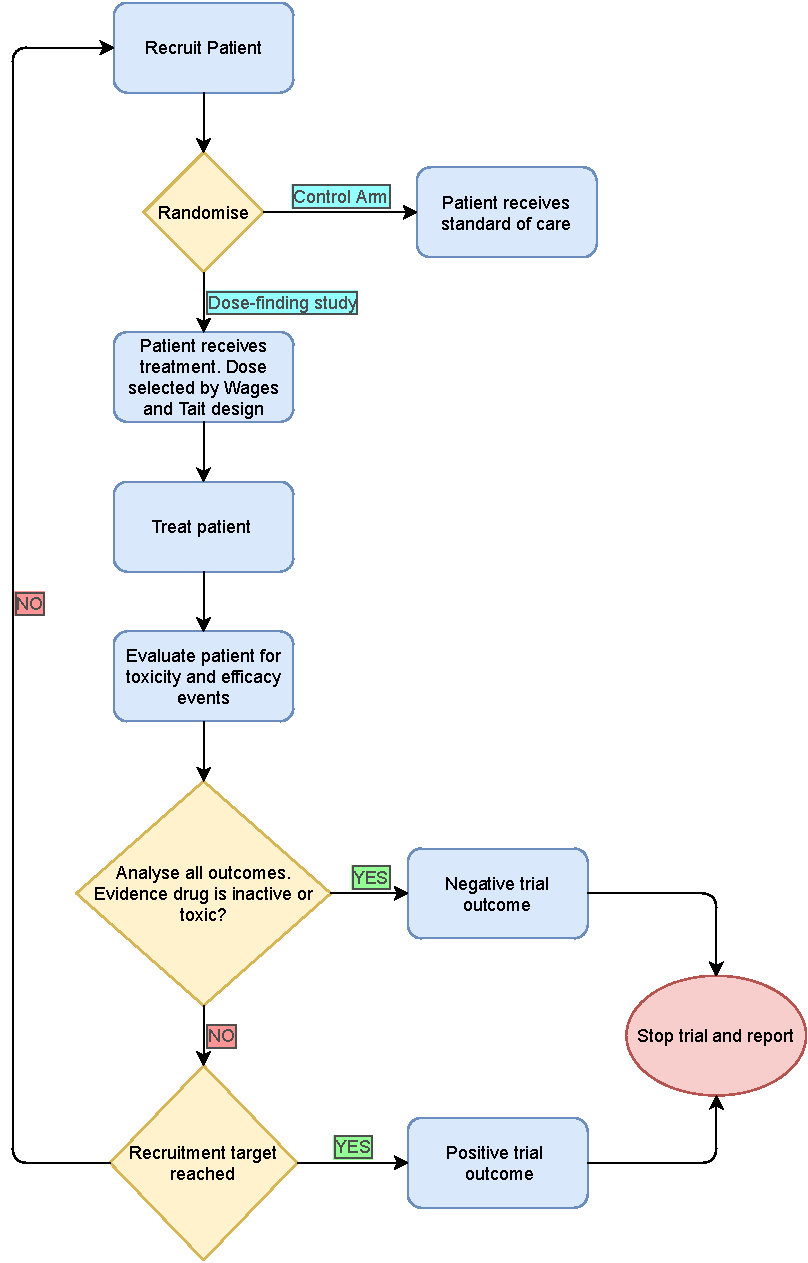
\includegraphics[width=0.77\textwidth]{WT-TwoArmExample}
\end{figure}

There is another approach which could also be used to include a control arm rather than our proposed design RtC-WT. A two arm randomised design could be used where patients are allocated to either the control arm or the dose-finding arm. Those patients allocated in the dose-finding arm will then be apart of the WT design see Figure \ref{fig_wt:TwoArmExample}. This approach maintains many of the traditional qualities of a two-arm randomised trial. The number of patients in each arm can be specified this way we guarantee a minimum number of patients in our control arm. Also, the characteristics of patients in both arms are likely to be similar which would be beneficial when making comparisons between the two arms. A downside of this method is that the data for control patients is no longer included in the modelling process. Whilst control patients may still be observed for efficacious and toxic events these won't be included in the modelling as such the ability to make inferences on the dose-toxicity and efficacy relationships in reference to a control/ standard of care dose is lost. 



Both of these approaches have their own merit but also have flaws as well. RtC-WT is somewhat of a middle ground which aims to recruit patients to a control dose and include the control patients data in the modelling process all whilst maintaining reasonable operating characteristics. We detail RtC-WT in Section \ref{WT:Design-RtC-WT} and explore the operating characteristics of this design in Section \ref{WT:Evaluation-of-the-Extension}.


%-----------------------------------
%	SUBSECTION 3.2
%-----------------------------------
\subsection{Design of the Proposed Extension RtC-WT}
\label{WT:Design-RtC-WT}

With this extension much of the Wages and Tait design stays the same. The modification only impacts the adaptive randomisation (AR) phase and requires some additional specification at the start of the trial. Firstly, we set the lowest dose-level $d_1$ to be the control dose-level. This dose-level should be included in the working models for efficacy and toxicity and should be treated like any other dose-level. Even if toxicity and efficacy events are expected to be non-existent for control its important that their corresponding skeleton values are non-zero. Investigators also need to consider a randomisation probability $\phi_R$ for the control dose. During the AR phase $\phi_R$ represents the probability of selecting the control dose as the next dose level. The probability of randomisation $R_i$ for other dose in $\mathscrsfs{A}_j$ is scaled accordingly such that the $\sum_{d_i \in \mathscrsfs{A}_j} R_i = 1$. The adaptive randomisation probabilities can now be expressed as 

\begin{equation}
R_1 = \phi_R
\end{equation}

\begin{equation}
R_i = (1-\phi_R)\frac{\hat{\pi}_E(d_i)}{\sum_{d_i \in \mathscrsfs{A}_j}\hat{\pi}_E(d_i)}, \; \; i=2,...,I. 
\end{equation}

Compared to Equation \ref{WT:eq_WT-ARprob} the adaptive randomisation probability is fixed to $\phi_R$ at the lowest dose (the control dose) and for all other dose levels in the admissible set $\mathscrsfs{A}_j$ a scaled randomisation probability is calculated. By fixing the probability for the control dose we guarantee a greater chance of patients being allocated to this dose-level. Although estimates of efficacy at the control dose-level $\hat{\pi}_E(d_1)$ do not directly impact its associated randomisation probability the efficacy data that generated the estimate is still included in the efficacy modelling and impacts probabilities for the remaining dose-levels. Also, by scaling the remaining probabilities of dose-levels in the admissible set we ensure that those doses with high estimates of efficacy maintain their proportional advantage of selection over the other non-control doses.

Some adjustments were made to the stopping rule for safety. The WT design assess the lower bound of the 95\% binomial confidence interval of the lowest dose to determine whether or not the trial should be stopped. However, with the RtC-WT design since the lowest dose is the control it makes little sense to surmise treatment is toxic here since non of the patients on control would have received the experimental treatment. It is also likely the trial would never recommend stopping even if the treatment is toxic since patients on control are likely to experience a toxic event. The RtC-WT design stops for safety by checking for excess toxicity at the second lowest dose-level (the first no contol dose-level). 

Once the AR phase ends dose-levels are no longer selected by adaptive randomisation. At this point it will be difficult for patients to be recruited to the control dose since recommended doses will be based on those with the greatest estimates of efficacy. As such it is important to consider the values set for both your randomisation probability for control $\phi_R$ and the size of the AR phase $j_R$. Wages and Tait simply suggest a 50:50 split between both the AR phase and the maximisation phase and show relatively good performance at this level. However, for RtC-WT the AR phase is the main component and more thought should be given here. In the next section we explore multiple combinations to better understand how these choices impact the operating characteristics of the design. We also compare RtC-WT to the two alternative designs mentioned in section  \ref{WT:Rationale-for-RtC-WT} via simulations and the inspection of operating characteristics specifically, selection probability of the OBD and patient allocation numbers at each dose-level. 
 
 
 %----------------------------------------------------------------------------------------
 %	SECTION 4
 %----------------------------------------------------------------------------------------
 \section{Evaluation and Exploration of the Extension via Simulations}
 \label{WT:Evaluation-of-the-Extension}
 
 In this section we evaluate the performance of RtC-WT in comparison to the two alternative designs mentioned in Section \ref{WT:Rationale-for-RtC-WT}. We also explore the impact of changing the probability of randomisation to control and the number of patients included in the adaptive randomisation phase. These will both be assessed via simulation and inspection of their operating characteristics. To facilitate simulations a generic trial example will be utilised along with a variety of scenarios. 
 
 %-----------------------------------
 %	SUBSECTION 4.1
 %-----------------------------------
 \subsection{Design Specification}
 \label{WT:Design-Spec}
 
 Here we detail the design specifications for RtC-WT that we will be using throughout this section. We assume five dose-levels, where the lowest dose is considered to be the control dose-level. The maximum sample size of the trial is set at 60 with patients recruited in cohorts of three and the first cohort starting at dose-level two (the first treatment dose-level). The pre-specified toxicity upper bound and efficacy lower bound are set at $\phi_T = 0.35$ and $\phi_E = 0.15$ respectively. Toxicity and efficacy skeletons are presented in table \ref{tab_wt:tox-eff-skeleton}. In terms of efficacy-relationships monotonic, unimodal and plateau skeletons were all used. We assume that each of the seven efficacy skeletons are equally likely and set $\upsilon(k) = \frac{1}{7}$. 
 

 \begin{table}[!h]
 	\centering
 	\caption{Toxicity and Efficacy skeletons for RtC-WT in the example trial.}
 	\label{tab_wt:tox-eff-skeleton}
 	\begin{tabular}{c|ccccc}
 		\hline
 		\multicolumn{1}{c|}{\multirow{2}{*}{\textbf{Skeleton}}} & \multicolumn{5}{c}{\textbf{Dose-levels}}                       \\
 		\multicolumn{1}{c|}{}                                   & \textbf{1} & \textbf{2} & \textbf{3} & \textbf{4} & \textbf{5} \\ \hline
 		$p_i$    & 0.01 & 0.1 & 0.2 & 0.3 & 0.4 \\
 		$q_{i1}$ & 0.01 & 0.4 & 0.3 & 0.2 & 0.1 \\
 		$q_{i2}$ & 0.01 & 0.3 & 0.4 & 0.3 & 0.2 \\
 		$q_{i3}$ & 0.01 & 0.2 & 0.3 & 0.4 & 0.3 \\
 		$q_{i4}$ & 0.01 & 0.1 & 0.2 & 0.3 & 0.4 \\
 		$q_{i5}$ & 0.01 & 0.2 & 0.3 & 0.4 & 0.4 \\
 		$q_{i6}$ & 0.01 & 0.3 & 0.4 & 0.4 & 0.4 \\
 		$q_{i7}$ & 0.01 & 0.4 & 0.4 & 0.4 & 0.4 \\ \hline
 	\end{tabular}
 \end{table}
 
 For the control dose we have set our prior beliefs to be very low for both toxicity and efficacy. This can of course be adapted if there is reason to believe that the control dose may be slightly more effective or toxic. Wages and Tait recommend $(2I-1)$ efficacy skeletons be used which in this example would be nine, however we have only considered seven. Since we don't expect many efficacy events from our lowest dose we dismiss the two extra efficacy skeletons as the dose-efficacy relationship they represent would be unlikely to occur. For completeness the first extra skeleton would be unimodal with the highest efficacy occurring at dose-level one and the second skeleton would be a plateau relationship with the plateau beginning at dose-level one as well. As with the values we've used for control these additional skeletons can also be incorporated if there is reason to believe so. 
 
 We also include the same stopping rules for safety and futility with the safety rule assessing toxicity at dose-level two. A rule will also be implemented to prevent the skipping of untried doses when escalating. This rule does not apply when de-escalating. 
 
 The two parameters we have left to specify are the fixed adaptive randomisation probability for control $\phi_R$ and the number of patients included in the adaptive randomisation phase $j_R$. In Section \ref{WT:Design-RtC-WT} we briefly the discus the importance of giving thought when setting these values. This is due to the fact they are the main things driving how RtC-WT works comparatively to the WT design. For example one could set the AR phase to last for the whole trial and keep a relative low probability to randomise to control. Alternatively, the AR phase can be set for half the patients in the trial and a double the probability of randomisation could be used. These two approaches could allocate the same number of patients in the control arm but have differing operating characteristics. It could be hypothesised that by setting the AR phase for the whole trial you miss out on the maximisation phase where patients are allocated to the estimated most efficacious dose which could yield slightly worse operating characteristics. We explore different combinations of these parameters in the next section. 
 
 %-----------------------------------
 %	SUBSECTION 4.2
 %-----------------------------------
 \subsection{Impact of AR phase size and probability of randomisation to control on RtC-WT}
 \label{WT:Impact-ARandRTCon-RtC-WT}
 
 The impact of the probability of control to randomisation is fairly intuitive as $\phi_R$ increases the number of patients allocated in the control dose-level is likely to increase. However, this is is only in isolation without considering the size of the AR phase. Increasing the AR phase would also mean more patients are likely allocated to the control dose-level since the randomisation only occurs in the AR phase. The interest lies within the interaction of both of these components and their impacts on operating characteristics. In order to gain a better understanding of this impact on RtC-WT we consider multiple of their possible combinations. 
 
 We look at two different probabilities for randomisation to control, $\phi_R = 0.2$ and $\phi_R = 0.4$ i.e. 20\% and 40\% probability of patients being allocated to the control dose-level during the AR phase of the trial. We also consider varying AR phase sizes, specifically $j_R = 0, 15, 30, 45 ,60$ essentially looking at when the AR phase lasts 0\%, 25\%, 50\%, 75\% and 100\% of the trial. The inclusion of setting the AR phase as 0 is somewhat counter-intuitive since the trial will just be run using the maximisation phase where the most efficacious doses are allocated. As such it is unlikely that the control dose-level would ever be the most efficacious specifically in our scenario here. However its inclusion will serve as a benchmark as the design most likely to achieve optimal performance in terms of locating the OBD since there will be no randomisation and the most efficacious dose will always be the one being tested. Although, many more combinations could be explored this set of 10 provide a good basis for us to gain a better understanding of how RtC-WT works. It also helps us understand how best to optimise RtC-WT for comparisons with alternative designs later on.  
 
 To compare these different combinations we use simulations covering a wide range of scenarios. For each scenario we simulate 10000 trials each consisting of 60 patients recruited in cohorts of three. Patient outcomes for toxicity and efficacy are randomly sampled using true toxicity and true efficacy probabilities, these are assumed to be independent of each other. Dose-allocation decisions are made after each cohort of patients is simulated and then the subsequent cohort is allocated the recommended dose or the trial is stopped when recruitment is reached and if stopping rules are triggered. The rest of the design specification is as defined in Section \ref{WT:Design-Spec}. 
 
 These true toxicity and efficacy probabilities are manipulated to produce each scenario. Scenario 1 to 4 look at monotonically increasing efficacy and toxicity curves. Scenarios 1 and 2 consider effective doses whereas scenarios 3 and 4 concern ineffective doses. Similarly, scenarios 1 and 3 contain all tolerable doses whereas 2 and 4 doses are considered too toxic. Scenarios 5 to 8 show plateau efficacy curves with 5 and 6 plateauing at dose level three and 7 and 8 plateauing at dose level four. Scenarios 6 and 8 doses are also considered too toxic, whereas 5 and 7 are tolerable. Scenarios 9 to 12 show unimodal efficacy curves with 9 and 10 peaking at dose level three and 11 and 12 peaking at four. Scenarios 9 and 11 consider tolerable doses and 10 and 12 are toxic. Operating characteristics and the scenarios under investigation are given in Tables \ref{tab_wt:SelectProbCombos} and \ref{tab_wt:MeanNCombos}. The selection probabilities of each combination under each scenario are also given in Table \ref{tab_wt:SelectProbCombos}. The mean number of patients recruited to each dose-level for each scenario and combination is provided in Table \ref{tab_wt:MeanNCombos}.  
 
\begin{table}
	
	\caption[Selection probabilities for multiple combinations of parameters.]{\label{tab_wt:SelectProbCombos}Selection probabilities for multiple combinations of AR phase size and probabilities for randomisation to control.}
	\centering
	\resizebox{\linewidth}{!}{
		\fontsize{9}{11}\selectfont
		\begin{tabular}[t]{cccccccc>{}c|ccccccccc}
			\toprule
			Scenario & $\phi_R$ & $j_R$ & Dose 1 & Dose 2 & Dose 3 & Dose 4 & Dose 5 & Stop & Scenario & $\phi_R$ & $j_R$ & Dose 1 & Dose 2 & Dose 3 & Dose 4 & Dose 5 & Stop\\
			\midrule
			P(tox) &  &  & 0.01 & 0.05 & 0.1 & 0.2 & 0.25 &  & P(tox) &  &  & 0.01 & 0.05 & 0.1 & 0.2 & 0.25 \vphantom{2} & \\
			\cmidrule{1-18}
			P(eff) &  &  & 0.01 & 0.25 & 0.35 & 0.45 & 0.55 &  & P(eff) &  &  & 0.01 & 0.25 & 0.35 & 0.55 & 0.55 \vphantom{1} & \\
			\cmidrule{1-18}
			& 0.2 & 0 & 0 & 0.28 & 0.28 & 0.21 & 0.23 & 0 &  & 0.2 & 0 & 0 & 0.28 & 0.2 & 0.3 & 0.22 & 0\\
			
			& 0.2 & 15 & 0 & 0.25 & 0.3 & 0.27 & 0.17 & 0 &  & 0.2 & 15 & 0 & 0.23 & 0.23 & 0.39 & 0.16 & 0\\
			
			& 0.2 & 30 & 0 & 0.18 & 0.28 & 0.34 & 0.21 & 0 &  & 0.2 & 30 & 0 & 0.14 & 0.18 & 0.5 & 0.18 & 0\\
			
			& 0.2 & 45 & 0 & 0.15 & 0.24 & 0.37 & 0.24 & 0 &  & 0.2 & 45 & 0 & 0.1 & 0.15 & 0.55 & 0.2 & 0\\
			
			& 0.2 & 60 & 0 & 0.15 & 0.2 & 0.36 & 0.29 & 0 &  & 0.2 & 60 & 0 & 0.09 & 0.13 & 0.51 & 0.26 & 0\\
			
			& 0.33 & 0 & 0 & 0.28 & 0.28 & 0.21 & 0.23 & 0 &  & 0.33 & 0 & 0 & 0.28 & 0.2 & 0.3 & 0.22 & 0\\
			
			& 0.33 & 15 & 0 & 0.26 & 0.33 & 0.25 & 0.16 & 0 &  & 0.33 & 15 & 0 & 0.25 & 0.25 & 0.36 & 0.13 & 0\\
			
			& 0.33 & 30 & 0 & 0.2 & 0.3 & 0.33 & 0.17 & 0 &  & 0.33 & 30 & 0 & 0.16 & 0.21 & 0.48 & 0.14 & 0\\
			
			& 0.33 & 45 & 0 & 0.16 & 0.27 & 0.37 & 0.2 & 0 &  & 0.33 & 45 & 0 & 0.12 & 0.18 & 0.53 & 0.16 & 0\\
			
			\multirow{-10}{*}{\centering\arraybackslash 1} & 0.33 & 60 & 0 & 0.18 & 0.23 & 0.38 & 0.22 & 0 & \multirow{-10}{*}{\centering\arraybackslash 7} & 0.33 & 60 & 0 & 0.14 & 0.17 & 0.51 & 0.19 & 0\\
			\cmidrule{1-18}
			P(tox) &  &  & 0.01 & 0.5 & 0.55 & 0.65 & 0.75 &  & P(tox) &  &  & 0.01 & 0.5 & 0.55 & 0.65 & 0.75 \vphantom{2} & \\
			\cmidrule{1-18}
			P(eff) &  &  & 0.01 & 0.25 & 0.35 & 0.45 & 0.55 &  & P(eff) &  &  & 0.01 & 0.25 & 0.35 & 0.55 & 0.55 & \\
			\cmidrule{1-18}
			& 0.2 & 0 & 0.07 & 0.15 & 0 & 0 & 0 & 0.77 &  & 0.2 & 0 & 0.07 & 0.15 & 0 & 0 & 0 & 0.78\\
			
			& 0.2 & 15 & 0.07 & 0.15 & 0 & 0 & 0 & 0.78 &  & 0.2 & 15 & 0.07 & 0.16 & 0 & 0 & 0 & 0.77\\
			
			& 0.2 & 30 & 0.07 & 0.16 & 0 & 0 & 0 & 0.78 &  & 0.2 & 30 & 0.07 & 0.15 & 0 & 0 & 0 & 0.78\\
			
			& 0.2 & 45 & 0.06 & 0.18 & 0 & 0 & 0 & 0.76 &  & 0.2 & 45 & 0.06 & 0.18 & 0 & 0 & 0 & 0.76\\
			
			& 0.2 & 60 & 0.08 & 0.31 & 0 & 0 & 0 & 0.61 &  & 0.2 & 60 & 0.08 & 0.32 & 0 & 0 & 0 & 0.6\\
			
			& 0.33 & 0 & 0.07 & 0.15 & 0 & 0 & 0 & 0.77 &  & 0.33 & 0 & 0.07 & 0.15 & 0 & 0 & 0 & 0.78\\
			
			& 0.33 & 15 & 0.07 & 0.16 & 0 & 0 & 0 & 0.77 &  & 0.33 & 15 & 0.06 & 0.16 & 0 & 0 & 0 & 0.77\\
			
			& 0.33 & 30 & 0.06 & 0.17 & 0 & 0 & 0 & 0.77 &  & 0.33 & 30 & 0.06 & 0.16 & 0 & 0 & 0 & 0.78\\
			
			& 0.33 & 45 & 0.04 & 0.21 & 0 & 0 & 0 & 0.74 &  & 0.33 & 45 & 0.04 & 0.22 & 0 & 0 & 0 & 0.74\\
			
			\multirow{-10}{*}{\centering\arraybackslash 2} & 0.33 & 60 & 0.04 & 0.38 & 0.01 & 0 & 0 & 0.57 & \multirow{-10}{*}{\centering\arraybackslash 8} & 0.33 & 60 & 0.04 & 0.37 & 0.01 & 0 & 0 & 0.58\\
			\cmidrule{1-18}
			P(tox) &  &  & 0.01 & 0.05 & 0.1 & 0.2 & 0.25 &  & P(tox) &  &  & 0.01 & 0.05 & 0.1 & 0.2 & 0.25 \vphantom{1} & \\
			\cmidrule{1-18}
			P(eff) &  &  & 0.01 & 0.03 & 0.06 & 0.09 & 0.12 &  & P(eff) &  &  & 0.01 & 0.35 & 0.55 & 0.35 & 0.25 \vphantom{1} & \\
			\cmidrule{1-18}
			& 0.2 & 0 & 0 & 0.03 & 0.12 & 0.28 & 0.36 & 0.21 &  & 0.2 & 0 & 0 & 0.32 & 0.58 & 0.09 & 0.01 & 0\\
			
			& 0.2 & 15 & 0 & 0.05 & 0.15 & 0.27 & 0.34 & 0.19 &  & 0.2 & 15 & 0 & 0.24 & 0.69 & 0.06 & 0.01 & 0\\
			
			& 0.2 & 30 & 0 & 0.08 & 0.19 & 0.31 & 0.31 & 0.12 &  & 0.2 & 30 & 0 & 0.19 & 0.74 & 0.06 & 0.01 & 0\\
			
			& 0.2 & 45 & 0 & 0.1 & 0.2 & 0.33 & 0.32 & 0.06 &  & 0.2 & 45 & 0 & 0.18 & 0.75 & 0.06 & 0 & 0\\
			
			& 0.2 & 60 & 0 & 0.13 & 0.18 & 0.31 & 0.37 & 0 &  & 0.2 & 60 & 0 & 0.23 & 0.7 & 0.07 & 0.01 & 0\\
			
			& 0.33 & 0 & 0 & 0.03 & 0.12 & 0.28 & 0.36 & 0.21 &  & 0.33 & 0 & 0 & 0.32 & 0.58 & 0.09 & 0.01 & 0\\
			
			& 0.33 & 15 & 0 & 0.05 & 0.15 & 0.29 & 0.34 & 0.17 &  & 0.33 & 15 & 0 & 0.27 & 0.66 & 0.06 & 0.01 & 0\\
			
			& 0.33 & 30 & 0 & 0.08 & 0.17 & 0.32 & 0.32 & 0.11 &  & 0.33 & 30 & 0 & 0.22 & 0.72 & 0.05 & 0.01 & 0\\
			
			& 0.33 & 45 & 0 & 0.12 & 0.19 & 0.33 & 0.32 & 0.05 &  & 0.33 & 45 & 0 & 0.22 & 0.71 & 0.06 & 0.01 & 0\\
			
			\multirow{-10}{*}{\centering\arraybackslash 3} & 0.33 & 60 & 0 & 0.14 & 0.18 & 0.32 & 0.36 & 0 & \multirow{-10}{*}{\centering\arraybackslash 9} & 0.33 & 60 & 0 & 0.26 & 0.66 & 0.07 & 0.01 & 0\\
			\cmidrule{1-18}
			P(tox) &  &  & 0.01 & 0.5 & 0.55 & 0.65 & 0.75 &  & P(tox) &  &  & 0.01 & 0.5 & 0.55 & 0.65 & 0.75 \vphantom{1} & \\
			\cmidrule{1-18}
			P(eff) &  &  & 0.01 & 0.03 & 0.06 & 0.09 & 0.12 &  & P(eff) &  &  & 0.01 & 0.35 & 0.55 & 0.35 & 0.25 & \\
			\cmidrule{1-18}
			& 0.2 & 0 & 0.01 & 0.03 & 0 & 0 & 0 & 0.96 &  & 0.2 & 0 & 0.07 & 0.15 & 0 & 0 & 0 & 0.78\\
			
			& 0.2 & 15 & 0.01 & 0.03 & 0 & 0 & 0 & 0.96 &  & 0.2 & 15 & 0.07 & 0.16 & 0 & 0 & 0 & 0.77\\
			
			& 0.2 & 30 & 0.01 & 0.03 & 0 & 0 & 0 & 0.95 &  & 0.2 & 30 & 0.07 & 0.16 & 0 & 0 & 0 & 0.78\\
			
			& 0.2 & 45 & 0.01 & 0.04 & 0 & 0 & 0 & 0.94 &  & 0.2 & 45 & 0.05 & 0.19 & 0 & 0 & 0 & 0.76\\
			
			& 0.2 & 60 & 0.08 & 0.32 & 0 & 0 & 0 & 0.6 &  & 0.2 & 60 & 0.07 & 0.31 & 0 & 0 & 0 & 0.61\\
			
			& 0.33 & 0 & 0.01 & 0.03 & 0 & 0 & 0 & 0.96 &  & 0.33 & 0 & 0.07 & 0.15 & 0 & 0 & 0 & 0.78\\
			
			& 0.33 & 15 & 0.02 & 0.03 & 0 & 0 & 0 & 0.95 &  & 0.33 & 15 & 0.07 & 0.16 & 0 & 0 & 0 & 0.77\\
			
			& 0.33 & 30 & 0.01 & 0.04 & 0 & 0 & 0 & 0.95 &  & 0.33 & 30 & 0.06 & 0.17 & 0 & 0 & 0 & 0.77\\
			
			& 0.33 & 45 & 0.01 & 0.05 & 0 & 0 & 0 & 0.93 &  & 0.33 & 45 & 0.04 & 0.22 & 0 & 0 & 0 & 0.74\\
			
			\multirow{-10}{*}{\centering\arraybackslash 4} & 0.33 & 60 & 0.05 & 0.37 & 0.01 & 0 & 0 & 0.57 & \multirow{-10}{*}{\centering\arraybackslash 10} & 0.33 & 60 & 0.04 & 0.37 & 0 & 0 & 0 & 0.58\\
			\cmidrule{1-18}
			P(tox) &  &  & 0.01 & 0.05 & 0.1 & 0.2 & 0.25 &  & P(tox) &  &  & 0.01 & 0.05 & 0.1 & 0.2 & 0.25 & \\
			\cmidrule{1-18}
			P(eff) &  &  & 0.01 & 0.35 & 0.55 & 0.55 & 0.55 &  & P(eff) &  &  & 0.01 & 0.25 & 0.35 & 0.55 & 0.35 \vphantom{1} & \\
			\cmidrule{1-18}
			& 0.2 & 0 & 0 & 0.31 & 0.44 & 0.16 & 0.09 & 0 &  & 0.2 & 0 & 0 & 0.29 & 0.21 & 0.45 & 0.05 & 0\\
			
			& 0.2 & 15 & 0 & 0.21 & 0.54 & 0.2 & 0.05 & 0 &  & 0.2 & 15 & 0 & 0.23 & 0.23 & 0.5 & 0.04 & 0\\
			
			& 0.2 & 30 & 0 & 0.13 & 0.53 & 0.28 & 0.06 & 0 &  & 0.2 & 30 & 0 & 0.15 & 0.2 & 0.62 & 0.04 & 0\\
			
			& 0.2 & 45 & 0 & 0.11 & 0.52 & 0.31 & 0.06 & 0 &  & 0.2 & 45 & 0 & 0.11 & 0.18 & 0.66 & 0.04 & 0\\
			
			& 0.2 & 60 & 0 & 0.15 & 0.45 & 0.33 & 0.08 & 0 &  & 0.2 & 60 & 0 & 0.11 & 0.17 & 0.63 & 0.09 & 0\\
			
			& 0.33 & 0 & 0 & 0.31 & 0.44 & 0.16 & 0.09 & 0 &  & 0.33 & 0 & 0 & 0.29 & 0.21 & 0.45 & 0.05 & 0\\
			
			& 0.33 & 15 & 0 & 0.23 & 0.55 & 0.17 & 0.04 & 0 &  & 0.33 & 15 & 0 & 0.26 & 0.26 & 0.44 & 0.04 & 0\\
			
			& 0.33 & 30 & 0 & 0.16 & 0.56 & 0.23 & 0.05 & 0 &  & 0.33 & 30 & 0 & 0.17 & 0.23 & 0.56 & 0.04 & 0\\
			
			& 0.33 & 45 & 0 & 0.14 & 0.55 & 0.26 & 0.05 & 0 &  & 0.33 & 45 & 0 & 0.13 & 0.22 & 0.6 & 0.04 & 0\\
			
			\multirow{-10}{*}{\centering\arraybackslash 5} & 0.33 & 60 & 0 & 0.21 & 0.48 & 0.26 & 0.05 & 0 & \multirow{-10}{*}{\centering\arraybackslash 11} & 0.33 & 60 & 0 & 0.15 & 0.2 & 0.57 & 0.08 & 0\\
			\cmidrule{1-18}
			P(tox) &  &  & 0.01 & 0.5 & 0.55 & 0.65 & 0.75 &  & P(tox) &  &  & 0.01 & 0.5 & 0.55 & 0.65 & 0.75 & \\
			\cmidrule{1-18}
			P(eff) &  &  & 0.01 & 0.35 & 0.55 & 0.55 & 0.55 &  & P(eff) &  &  & 0.01 & 0.25 & 0.35 & 0.55 & 0.35 & \\
			\cmidrule{1-18}
			& 0.2 & 0 & 0.07 & 0.15 & 0 & 0 & 0 & 0.78 &  & 0.2 & 0 & 0.07 & 0.15 & 0 & 0 & 0 & 0.78\\
			
			& 0.2 & 15 & 0.07 & 0.16 & 0 & 0 & 0 & 0.77 &  & 0.2 & 15 & 0.07 & 0.16 & 0 & 0 & 0 & 0.77\\
			
			& 0.2 & 30 & 0.07 & 0.16 & 0 & 0 & 0 & 0.77 &  & 0.2 & 30 & 0.07 & 0.15 & 0 & 0 & 0 & 0.78\\
			
			& 0.2 & 45 & 0.05 & 0.19 & 0 & 0 & 0 & 0.76 &  & 0.2 & 45 & 0.06 & 0.18 & 0 & 0 & 0 & 0.76\\
			
			& 0.2 & 60 & 0.07 & 0.32 & 0 & 0 & 0 & 0.61 &  & 0.2 & 60 & 0.08 & 0.32 & 0 & 0 & 0 & 0.6\\
			
			& 0.33 & 0 & 0.07 & 0.15 & 0 & 0 & 0 & 0.78 &  & 0.33 & 0 & 0.07 & 0.15 & 0 & 0 & 0 & 0.78\\
			
			& 0.33 & 15 & 0.07 & 0.16 & 0 & 0 & 0 & 0.77 &  & 0.33 & 15 & 0.06 & 0.16 & 0 & 0 & 0 & 0.77\\
			
			& 0.33 & 30 & 0.06 & 0.17 & 0 & 0 & 0 & 0.77 &  & 0.33 & 30 & 0.06 & 0.16 & 0 & 0 & 0 & 0.78\\
			
			& 0.33 & 45 & 0.04 & 0.22 & 0 & 0 & 0 & 0.74 &  & 0.33 & 45 & 0.04 & 0.22 & 0 & 0 & 0 & 0.74\\
			
			\multirow{-10}{*}{\centering\arraybackslash 6} & 0.33 & 60 & 0.04 & 0.37 & 0.01 & 0 & 0 & 0.58 & \multirow{-10}{*}{\centering\arraybackslash 12} & 0.33 & 60 & 0.04 & 0.37 & 0.01 & 0 & 0 & 0.58\\
			\bottomrule
	\end{tabular}}
\end{table}

\begin{table}
	
	\caption[Mean No. of patients for multiple combinations of parameters.]{\label{tab_wt:MeanNCombos}Mean number of patients treated at each dose for multiple combinations of AR phase size and probabilities for randomisation to control.}
	\centering
	\resizebox{\linewidth}{!}{
		\fontsize{9}{11}\selectfont
		\begin{tabular}[t]{cccccccc>{}c|ccccccccc}
			\toprule
			Scenario & $\phi_R$ & $j_R$ & Dose 1 & Dose 2 & Dose 3 & Dose 4 & Dose 5 & Total & Scenario & $\phi_R$ & $j_R$ & Dose 1 & Dose 2 & Dose 3 & Dose 4 & Dose 5 & Total\\
			\midrule
			P(tox) &  &  & 0.01 & 0.05 & 0.1 & 0.2 & 0.25 &  & P(tox) &  &  & 0.01 & 0.05 & 0.1 & 0.2 & 0.25 \vphantom{2} & \\
			\cmidrule{1-18}
			P(eff) &  &  & 0.01 & 0.25 & 0.35 & 0.45 & 0.55 &  & P(eff) &  &  & 0.01 & 0.25 & 0.35 & 0.55 & 0.55 \vphantom{1} & \\
			\cmidrule{1-18}
			& 0.2 & 0 & 0.1 & 21.1 & 16.9 & 11.2 & 10.7 & 60 &  & 0.2 & 0 & 0.1 & 20.9 & 13.9 & 14.3 & 10.8 & 60\\
			
			& 0.2 & 15 & 2.4 & 18.3 & 18 & 13.6 & 7.6 & 59.9 &  & 0.2 & 15 & 2.4 & 17.1 & 15.3 & 17.9 & 7.2 & 59.9\\
			
			& 0.2 & 30 & 5.5 & 14.9 & 16 & 15.4 & 8.2 & 60 &  & 0.2 & 30 & 5.4 & 13.9 & 13.5 & 19.5 & 7.7 & 60\\
			
			& 0.2 & 45 & 8.5 & 14.2 & 14.7 & 14.4 & 8.2 & 60 &  & 0.2 & 45 & 8.5 & 13.4 & 13.5 & 16.9 & 7.7 & 60\\
			
			& 0.2 & 60 & 11.4 & 14.3 & 14.4 & 12.6 & 7.3 & 60 &  & 0.2 & 60 & 11.4 & 13.9 & 14.3 & 12.9 & 7.5 & 60\\
			
			& 0.33 & 0 & 0.1 & 21.1 & 16.9 & 11.2 & 10.7 & 60 &  & 0.33 & 0 & 0.1 & 20.9 & 13.9 & 14.3 & 10.8 & 60\\
			
			& 0.33 & 15 & 4 & 18.4 & 18.4 & 12.6 & 6.6 & 60 &  & 0.33 & 15 & 4 & 18 & 16 & 16.1 & 5.9 & 60\\
			
			& 0.33 & 30 & 9 & 14.9 & 15.7 & 13.9 & 6.4 & 59.9 &  & 0.33 & 30 & 9 & 13.8 & 13.7 & 17.7 & 5.8 & 60\\
			
			& 0.33 & 45 & 13.9 & 13.2 & 13.8 & 12.7 & 6.3 & 59.9 &  & 0.33 & 45 & 13.9 & 12.4 & 12.6 & 15.1 & 6 & 60\\
			
			\multirow{-10}{*}{\centering\arraybackslash 1} & 0.33 & 60 & 19 & 12.7 & 12.6 & 10.4 & 5.4 & 60.1 & \multirow{-10}{*}{\centering\arraybackslash 7} & 0.33 & 60 & 18.9 & 12.5 & 12.5 & 10.6 & 5.5 & 60\\
			\cmidrule{1-18}
			P(tox) &  &  & 0.01 & 0.5 & 0.55 & 0.65 & 0.75 &  & P(tox) &  &  & 0.01 & 0.5 & 0.55 & 0.65 & 0.75 \vphantom{2} & \\
			\cmidrule{1-18}
			P(eff) &  &  & 0.01 & 0.25 & 0.35 & 0.45 & 0.55 &  & P(eff) &  &  & 0.01 & 0.25 & 0.35 & 0.55 & 0.55 & \\
			\cmidrule{1-18}
			& 0.2 & 0 & 15.3 & 23.2 & 0.7 & 0.1 & 0 & 39.3 &  & 0.2 & 0 & 15.2 & 23.1 & 0.7 & 0.1 & 0 & 39.1\\
			
			& 0.2 & 15 & 15.3 & 22.8 & 1 & 0.1 & 0 & 39.2 &  & 0.2 & 15 & 15.3 & 22.8 & 1 & 0.1 & 0 & 39.2\\
			
			& 0.2 & 30 & 15.5 & 22.6 & 1 & 0.1 & 0 & 39.2 &  & 0.2 & 30 & 15.4 & 22.4 & 0.9 & 0.1 & 0 & 38.8\\
			
			& 0.2 & 45 & 16.5 & 23 & 1 & 0.1 & 0 & 40.6 &  & 0.2 & 45 & 16.5 & 22.9 & 1 & 0.1 & 0 & 40.5\\
			
			& 0.2 & 60 & 17.8 & 22.6 & 1 & 0.1 & 0 & 41.5 &  & 0.2 & 60 & 17.9 & 22.8 & 1 & 0.1 & 0 & 41.8\\
			
			& 0.33 & 0 & 15.3 & 23.2 & 0.7 & 0.1 & 0 & 39.3 &  & 0.33 & 0 & 15.2 & 23.1 & 0.7 & 0.1 & 0 & 39.1\\
			
			& 0.33 & 15 & 15.5 & 22.7 & 1.1 & 0.1 & 0 & 39.4 &  & 0.33 & 15 & 15.5 & 22.7 & 1.2 & 0.1 & 0 & 39.5\\
			
			& 0.33 & 30 & 16 & 22.5 & 1.4 & 0.1 & 0 & 40 &  & 0.33 & 30 & 15.9 & 22.3 & 1.3 & 0.1 & 0 & 39.6\\
			
			& 0.33 & 45 & 17.5 & 22.2 & 1.3 & 0.1 & 0 & 41.1 &  & 0.33 & 45 & 17.3 & 22.1 & 1.3 & 0.1 & 0 & 40.8\\
			
			\multirow{-10}{*}{\centering\arraybackslash 2} & 0.33 & 60 & 20 & 21.4 & 1.3 & 0.1 & 0 & 42.8 & \multirow{-10}{*}{\centering\arraybackslash 8} & 0.33 & 60 & 19.9 & 21.4 & 1.3 & 0.1 & 0 & 42.7\\
			\cmidrule{1-18}
			P(tox) &  &  & 0.01 & 0.05 & 0.1 & 0.2 & 0.25 &  & P(tox) &  &  & 0.01 & 0.05 & 0.1 & 0.2 & 0.25 \vphantom{1} & \\
			\cmidrule{1-18}
			P(eff) &  &  & 0.01 & 0.03 & 0.06 & 0.09 & 0.12 &  & P(eff) &  &  & 0.01 & 0.35 & 0.55 & 0.35 & 0.25 \vphantom{1} & \\
			\cmidrule{1-18}
			& 0.2 & 0 & 0.1 & 9.7 & 11.3 & 17.5 & 18.9 & 57.5 &  & 0.2 & 0 & 0.1 & 26.4 & 27.1 & 5.2 & 1.2 & 60\\
			
			& 0.2 & 15 & 2.4 & 10.7 & 12.3 & 16.2 & 16.3 & 57.9 &  & 0.2 & 15 & 2.4 & 18.7 & 32.5 & 5.4 & 0.9 & 59.9\\
			
			& 0.2 & 30 & 5.4 & 11.1 & 13.7 & 15.9 & 12.9 & 59 &  & 0.2 & 30 & 5.4 & 16.6 & 28.3 & 7.6 & 2 & 59.9\\
			
			& 0.2 & 45 & 8.4 & 11.3 & 13.6 & 15.2 & 11.2 & 59.7 &  & 0.2 & 45 & 8.4 & 16.2 & 22.3 & 9.5 & 3.5 & 59.9\\
			
			& 0.2 & 60 & 11.5 & 11.1 & 13.7 & 14.3 & 9.4 & 60 &  & 0.2 & 60 & 11.5 & 16.1 & 15.6 & 11.6 & 5.3 & 60.1\\
			
			& 0.33 & 0 & 0.1 & 9.7 & 11.3 & 17.5 & 18.9 & 57.5 &  & 0.33 & 0 & 0.1 & 26.4 & 27.1 & 5.2 & 1.2 & 60\\
			
			& 0.33 & 15 & 4 & 10.2 & 11.8 & 15.9 & 16.3 & 58.2 &  & 0.33 & 15 & 4 & 19.6 & 30.8 & 4.9 & 0.8 & 60.1\\
			
			& 0.33 & 30 & 9 & 10.4 & 12.2 & 15.2 & 12.4 & 59.2 &  & 0.33 & 30 & 8.9 & 16.4 & 26.6 & 6.5 & 1.6 & 60\\
			
			& 0.33 & 45 & 13.8 & 10.4 & 12.3 & 13.6 & 9.8 & 59.9 &  & 0.33 & 45 & 13.9 & 15.3 & 20 & 8.1 & 2.7 & 60\\
			
			\multirow{-10}{*}{\centering\arraybackslash 3} & 0.33 & 60 & 19 & 10 & 12.1 & 11.8 & 7.1 & 60 & \multirow{-10}{*}{\centering\arraybackslash 9} & 0.33 & 60 & 19 & 14.1 & 13.3 & 9.6 & 4 & 60\\
			\cmidrule{1-18}
			P(tox) &  &  & 0.01 & 0.5 & 0.55 & 0.65 & 0.75 &  & P(tox) &  &  & 0.01 & 0.5 & 0.55 & 0.65 & 0.75 \vphantom{1} & \\
			\cmidrule{1-18}
			P(eff) &  &  & 0.01 & 0.03 & 0.06 & 0.09 & 0.12 &  & P(eff) &  &  & 0.01 & 0.35 & 0.55 & 0.35 & 0.25 & \\
			\cmidrule{1-18}
			& 0.2 & 0 & 13.3 & 18.4 & 1.1 & 0.2 & 0 & 33 &  & 0.2 & 0 & 15.3 & 23.3 & 0.5 & 0 & 0 & 39.1\\
			
			& 0.2 & 15 & 13.3 & 18.2 & 1.3 & 0.2 & 0 & 33 &  & 0.2 & 15 & 15.2 & 22.9 & 1 & 0.1 & 0 & 39.2\\
			
			& 0.2 & 30 & 14.2 & 18.7 & 1.2 & 0.1 & 0 & 34.2 &  & 0.2 & 30 & 15.6 & 22.7 & 0.9 & 0.1 & 0 & 39.3\\
			
			& 0.2 & 45 & 16.2 & 20.9 & 1.2 & 0.2 & 0 & 38.5 &  & 0.2 & 45 & 16.5 & 23 & 1 & 0.1 & 0 & 40.6\\
			
			& 0.2 & 60 & 18.1 & 22.8 & 1.2 & 0.1 & 0 & 42.2 &  & 0.2 & 60 & 17.9 & 22.7 & 0.9 & 0.1 & 0 & 41.6\\
			
			& 0.33 & 0 & 13.3 & 18.4 & 1.1 & 0.2 & 0 & 33 &  & 0.33 & 0 & 15.3 & 23.3 & 0.5 & 0 & 0 & 39.1\\
			
			& 0.33 & 15 & 13.6 & 18.3 & 1.5 & 0.2 & 0 & 33.6 &  & 0.33 & 15 & 15.4 & 23 & 1 & 0.1 & 0 & 39.5\\
			
			& 0.33 & 30 & 14.8 & 18.5 & 1.6 & 0.2 & 0 & 35.1 &  & 0.33 & 30 & 16 & 22.5 & 1.3 & 0.1 & 0 & 39.9\\
			
			& 0.33 & 45 & 17.1 & 19.8 & 1.5 & 0.2 & 0 & 38.6 &  & 0.33 & 45 & 17.6 & 22.4 & 1.3 & 0.1 & 0 & 41.4\\
			
			\multirow{-10}{*}{\centering\arraybackslash 4} & 0.33 & 60 & 19.9 & 21 & 1.5 & 0.2 & 0 & 42.6 & \multirow{-10}{*}{\centering\arraybackslash 10} & 0.33 & 60 & 19.9 & 21.5 & 1.2 & 0.1 & 0 & 42.7\\
			\cmidrule{1-18}
			P(tox) &  &  & 0.01 & 0.05 & 0.1 & 0.2 & 0.25 &  & P(tox) &  &  & 0.01 & 0.05 & 0.1 & 0.2 & 0.25 & \\
			\cmidrule{1-18}
			P(eff) &  &  & 0.01 & 0.35 & 0.55 & 0.55 & 0.55 &  & P(eff) &  &  & 0.01 & 0.25 & 0.35 & 0.55 & 0.35 \vphantom{1} & \\
			\cmidrule{1-18}
			& 0.2 & 0 & 0.1 & 26.1 & 21.7 & 7.4 & 4.8 & 60.1 &  & 0.2 & 0 & 0.1 & 21.3 & 14.4 & 19.5 & 4.8 & 60.1\\
			
			& 0.2 & 15 & 2.5 & 17.2 & 27 & 10.6 & 2.7 & 60 &  & 0.2 & 15 & 2.4 & 17.1 & 15.6 & 21.4 & 3.4 & 59.9\\
			
			& 0.2 & 30 & 5.4 & 14.3 & 22.6 & 13.7 & 4 & 60 &  & 0.2 & 30 & 5.4 & 13.9 & 14.3 & 22.4 & 4 & 60\\
			
			& 0.2 & 45 & 8.5 & 14.3 & 18.6 & 13.4 & 5.2 & 60 &  & 0.2 & 45 & 8.4 & 13.7 & 14.1 & 18.4 & 5.3 & 59.9\\
			
			& 0.2 & 60 & 11.4 & 14.9 & 14.7 & 12.3 & 6.6 & 59.9 &  & 0.2 & 60 & 11.5 & 14.3 & 14.5 & 12.8 & 6.8 & 59.9\\
			
			& 0.33 & 0 & 0.1 & 26.1 & 21.7 & 7.4 & 4.8 & 60.1 &  & 0.33 & 0 & 0.1 & 21.3 & 14.4 & 19.5 & 4.8 & 60.1\\
			
			& 0.33 & 15 & 4 & 17.8 & 27 & 9 & 2.2 & 60 &  & 0.33 & 15 & 4 & 18.2 & 16.3 & 18.5 & 3 & 60\\
			
			& 0.33 & 30 & 9 & 14.4 & 22.5 & 11.3 & 2.9 & 60.1 &  & 0.33 & 30 & 9 & 13.9 & 14.3 & 19.5 & 3.3 & 60\\
			
			& 0.33 & 45 & 13.8 & 13.7 & 17.5 & 11.1 & 3.9 & 60 &  & 0.33 & 45 & 13.9 & 12.9 & 13 & 15.9 & 4.3 & 60\\
			
			\multirow{-10}{*}{\centering\arraybackslash 5} & 0.33 & 60 & 18.9 & 13.3 & 12.7 & 10 & 5 & 59.9 & \multirow{-10}{*}{\centering\arraybackslash 11} & 0.33 & 60 & 18.9 & 12.6 & 12.6 & 10.6 & 5.3 & 60\\
			\cmidrule{1-18}
			P(tox) &  &  & 0.01 & 0.5 & 0.55 & 0.65 & 0.75 &  & P(tox) &  &  & 0.01 & 0.5 & 0.55 & 0.65 & 0.75 & \\
			\cmidrule{1-18}
			P(eff) &  &  & 0.01 & 0.35 & 0.55 & 0.55 & 0.55 &  & P(eff) &  &  & 0.01 & 0.25 & 0.35 & 0.55 & 0.35 & \\
			\cmidrule{1-18}
			& 0.2 & 0 & 15.4 & 23.3 & 0.5 & 0.1 & 0 & 39.3 &  & 0.2 & 0 & 15.3 & 23.1 & 0.7 & 0.1 & 0 & 39.2\\
			
			& 0.2 & 15 & 15.2 & 22.8 & 1 & 0.1 & 0 & 39.1 &  & 0.2 & 15 & 15.3 & 22.8 & 1 & 0.1 & 0 & 39.2\\
			
			& 0.2 & 30 & 15.6 & 22.8 & 1 & 0.1 & 0 & 39.5 &  & 0.2 & 30 & 15.4 & 22.4 & 0.9 & 0.1 & 0 & 38.8\\
			
			& 0.2 & 45 & 16.4 & 23 & 0.9 & 0.1 & 0 & 40.4 &  & 0.2 & 45 & 16.5 & 22.9 & 1 & 0.1 & 0 & 40.5\\
			
			& 0.2 & 60 & 18 & 22.8 & 0.9 & 0.1 & 0 & 41.8 &  & 0.2 & 60 & 17.9 & 22.8 & 1 & 0.1 & 0 & 41.8\\
			
			& 0.33 & 0 & 15.4 & 23.3 & 0.5 & 0.1 & 0 & 39.3 &  & 0.33 & 0 & 15.3 & 23.1 & 0.7 & 0.1 & 0 & 39.2\\
			
			& 0.33 & 15 & 15.3 & 22.9 & 1 & 0.1 & 0 & 39.3 &  & 0.33 & 15 & 15.5 & 22.7 & 1.2 & 0.1 & 0 & 39.5\\
			
			& 0.33 & 30 & 15.9 & 22.5 & 1.2 & 0.1 & 0 & 39.7 &  & 0.33 & 30 & 15.9 & 22.3 & 1.3 & 0.1 & 0 & 39.6\\
			
			& 0.33 & 45 & 17.7 & 22.6 & 1.3 & 0.1 & 0 & 41.7 &  & 0.33 & 45 & 17.3 & 22.1 & 1.3 & 0.1 & 0 & 40.8\\
			
			\multirow{-10}{*}{\centering\arraybackslash 6} & 0.33 & 60 & 19.9 & 21.5 & 1.2 & 0.1 & 0 & 42.7 & \multirow{-10}{*}{\centering\arraybackslash 12} & 0.33 & 60 & 19.9 & 21.4 & 1.3 & 0.1 & 0 & 42.7\\
			\bottomrule
	\end{tabular}}
\end{table}

For scenario 1 it is relatively simple to select an admissible dose since all doses are tolerable and efficacy increases monotonically. The difficulty is locating the OBD. All of these combinations fail to identify the OBD (dose-level 5) more than 30\% of the time. As the size of the AR phase increases from 15 to 60 so do the selection probabilities, going from 17\% to 29\% and 16\% to 22\% for randomisation probabilities of 0.2 and 0.33 respectively. Overall, the designs with higher probability of randomising to control fair slightly worse. In the case of no AR phase, $j_R =0$, the design is roughly selects all active doses (dose-levels 2 to 5) at a similar rate, slightly preferring the lower dose levels. It should be noted that the two designs with no AR phase are identical since the randomisation probabilities are never used. In terms of numbers of patients treated we see more patients in the control arm as AR phase size and randomisation probability increase. This is expected since if you increase the amount of time available for cohorts to be randomised or the probability in which that is done so more patients will be recruited to control. By increasing the probability of randomising to control we can also see that less patients are being treated at the optimal dose. Also, the $\phi_R$ figure does not guarantee that exact percentage of patients in the control dose. On average these values seem to be less than one patient off. 

Scenario 2 has no OBD as all treatment doses are considered toxic. For most of the combinations stopping occurs 74-78\% of the time. Slightly concerning is the case where the AR phase lasts the whole trial. Here stopping is less frequent at 61\% and 57\% for doses $\phi_R = 0.2$ and $\phi_R = 0.33$ respectively. One reason why this may occur is that early on during the trial it will be difficult to discern the toxic dose-levels with low numbers of patients and since these designs don't activate the maximisation phase they will constonatly be allocating patients to control. As such it may be the case that not enough toxicity events are being collected to recommend to stop. Interestingly when you look at the average number of patients allocated to control this is similar across the board, even for the case where no adaptive randomisation si taking place. This probably happens since non of the treatment dose-levels make it into the admissible set. If there is only one dose-level in the admissible set after modelling toxicity the design will automatically allocate to that dose.  

In scenario 3, the treatment is tolerable but the treatment effect is weak. Again there is no OBD and the trial should recommend stopping for futility. For designs where $j_R$ is set to the max sample size, in this case 60, stopping will never occur here. this is due to the fact there is no maximisation phase and consequently the futility stopping rule doesn't come into play. We can see those with smaller AR phase stop more often although not enough. Most of the time these designs are selecting dose-level 5 as the OBD since its true efficacy rate is somewhat close to the lower bound of efficacy. We can see the majority of patients being allocated to this dose-level as well. Since this dose is not toxic this seems reasonable but ideally it would be preferable if the designs recommended stopping. 

Scenario 4 is where the treatment is considered toxic and inefficacious. Compared to scenario 2 we see high probability of stopping (93\% - 96\%) approximately 20 \% higher for all of the combinations except where the size of the AR phase is the same as the whole trial. This will be due to the futility rule stopping the trial in instances where toxicity events aren't occurring but doses are still ineffective. 

Scenario 5 looks at a plateau relationship where dose-efficacy stops increasing after dose 3. Except for when the AR phase size is 0 or 60 the OBD is selected more than 50\% of the time. When the AR phase lasts the whole trial the design seems to run into the issue where dose levels 3, 4 and 5 are all admissible and equally efficacious as such the probability of randomising between these will be somewhat similar. The designs with no AR phase seem to get stuck at lower dose-levels since there is also some efficacious effect there. For both of these combinations we can see this reflected in the average patient numbers for each dose. Looking at the differences between the randomisation to control probabilities we see a minimal increase, approximately 1\% in selection of the OBD for $\phi_R = 0.33$. We also see slightly more patients treated at the OBD for lower numbers of $j_R$. This is most likely due to there being less randomisation and more allocation based on efficacy data once an initial set of data has been collected. 

Scenario 6 looks at a similar efficacy curve as scenario 5 but all doses are toxic. Once again, this behaves similarly to other toxic scenarios 2 and 4 where stopping occurs well except in the case where adaptive randomisation lasts the whole trial. 

Scenario 7 is similar to scenario 5 except the plateau begins at dose 4. Here the selection probabilities for small AR phases(0-15) fall off but increase fo 60 in comparison to scenario 5. For an AR phase size of 0 the design still gets stuck at the lower doses. Now with the plateau at 4 the OBD is one dose-level further away from the starting dose. Thus the designs with small AR phases are unable to randomise enough patients to higher dose levels and get stuck during their maximisation phase. Inversely this improved the performance for $j_R = 60$ as there is one less dose level with similar efficacy so the design has an easier time locating the OBD via randomisation. Scenario 8 involves the same efficacy relationship as scenario 7 except when all doses are toxic. Here we see similar performance as prior scenarios with toxic doses.  

Scenarios 9 and 11 look at unimodal efficacy relationships where the mos efficacious dose is at doses 3 and 4 respectively. Overall, we see much higher selection probabilities in these scenarios with those in 9 being slightly higher than those in 11. Similar to the plateau relationships we see less performance for those designs with $j_R = 0$ and  $j_R = 60$. With these scenarios we also see a slight increase in the average number of patients treated at the OBD. The increase in performance may be due to the fact that there is only one dose with a high level of efficacy whereas previous dose had multiple highly efficacious doses to allocate to. The impact of randomisation probabilities appear to be more apparent in scenario 11 where $\phi_R = 0.33$ designs have slightly lower performance. As with scenario 7 since the OBD is one dose further from the starting dose and more patients are being randomised to control there's less chance to obtain data on those higher doses through the initial randomisation in the AR phase. 

Finally, scenarios 10 and 12 look at the versions of scenario 9 and 11 respectively where all doses are toxic. Once again, similar characteristics are observed to other toxic scenarios. 

In general these scenarios show us that there are some issues with certain specifications of $\phi_R$ and $j_R$ in some of the scenarios presented. Specifically, in the case of stopping for toxicity, having the AR phase being the same as the sample size causes some issues. Also, an AR phase size of 0 does not perform well if the dose-efficacy relationship plateaus. For the randomisation probabilities performance was mostly similar between the two values we chose. Some difficulties were observed for higher probabilities of randomisation when the OBD is further away from the starting dose-level. In terms of patient numbers at the control dose we see on average a similar number, if not slightly lower, to what would be expected i.e. for $\phi_R = 0.2$ and  $j_R = 45$ you would expect 9 control patients (20\% of 45) our simulations yielded about 8.5 on average dependent on scenario. 

Based on these simulations it would be best to use an AR phase size between 25\% and 75\% of the total sample size and a randomisation to control probability that will produce the number of control patients you are interested in. However, it may be beneficial to investigate various values of $\phi_R$ as there does appear to be some trade-off in terms of performance and the number of patients recruited to th the control dose.




 %-----------------------------------
 %	SUBSECTION 4.3
 %-----------------------------------
 \subsection{Comparison of RtC-WT against Alternative Designs }
 \label{WT:CompAltDesigns}
 
 The simulations in the previous section were about exploring the impact of varying the parameters controlling the randomisation in RtC-WT. In this section we investigate two alternative trial approaches which could be used to achieve the same aims as RtC-WT, that is to conduct a dose-finding study locating the ODB whilst recruiting patients to a control arm. Simulations will be conducted for these two alternatives across a variety of scenarios and operating characteristics will be compared against those for RtC-WT.       
 
 The first alternative approach would be just to use a standard Wages and Tait design and include the lowest dose-level as control. We will refer to this approach as the standard Wages and Tait (WT). Technically this design doesn't aim to recruit control patients but by including it as a dose-level there is still a small probability during the AR phase that this occurs. Either way this will be a good comparator for RtC-WT as we will be able to directly compare how our extension impacts performance compared to a traditional Wages and Tait design. Theoretically since the standard Wages and Tait design won't be forced to allocate patients to the control dose-level you would expect more patients too be allocated at the experimental treatment dose-levels leading to more data on efficacy and toxicity relationships making it easier to locate the ODB. The differences in performance between these two designs could be considered as the cost for including a control dose. 
 
 The second design is one which uses a two-arm randomised approach. Patients once recruited are randomised to either a control arm or a dose-finding study arm. The dose-finding study-arm will use the method of Wages and Tait to identify a OBD. We will refer to this method as the two-arm approach. One of the benefits of this approach is that it is fairly simplistic. This could be considered as a straight-forward way of including a control arm into complex designs without having to figure out any complicated mathematics. For example, the EffTox design could be used for the dose-finding arm and due to the two-arm approach we now have a cohort of control patients without building that methodology directly into the design. For the dose-finding study any methodology could be used here to locate an OBD, however we selected WT to provide more comparisons for RtC-WT. Since the randomisation occurs up front a guaranteed number of patients can be expected in the control arm, which may be a desirable characteristic of this design. In terms of comparisons to RtC-WT this design will allow us to see if it is worth including the control patients directly in the dose-finding aspect of the design and if there's any benefit in terms of operating characteristics.  
 
 For RtC-WT we will be using the same design specification as detailed in Section \ref{WT:Design-Spec}. In terms of parameters for the number of patients in the AR phase and the probability of randomising to control these will be set at $j_R = 45 $ and $\phi_R = 0.2 $ respectively. These values were selected based on the work done in the previous section. This combination of parameters seemed to perform consistently across all the scenarios explored. The standard Wages and Tait approach will also be using the same specification except for the fixed probability of randomisation to control.
 
 For the two-arm approach things are slightly different since patients are being randomised first. Looking at the RtC-WT design we have specified a sample size of 60, an AR phase size of 45 and probability of randomising to control at 20\%. Here we would expect roughly nine patients to be allocated to the control arm (20\% of 45), looking at Table for this combo we see on average we achieve around 8.5 patients at the control dose-level. To mimic this behaviour for the two-arm approach we would need to specify a randomisation ratio upfront. Based on the parameters set for RtC-WT this can be done generally using the formula:
 
 \begin{equation}
 1 : \frac{J}{\phi_R j_r} - 1
 \end{equation}
 
 where $J$ is the maximum sample size. In this scenario this corresponds to a 1:5.67 (3:17) randomisation. So for the two-arm approach we will have 9 patients in control and 51 patients in the dose-finding study. 
 
 The specifications for the dose-finding study will be somewhat similar as well. Here there will only be four dose levels (no control dose-level) i.e doses 2-5 in Section \ref{WT:Design-Spec}. We also adjust the toxicity and efficacy skeletons accordingly in Table \ref{tab_wt:tox-eff-skeleton} as well by removing the values from dose-level 1. Since there is no control dose-level in the design we will just be using approximately 50\% of the patients in the AR phase, as recommended by Wages and Tait. As there will be 51 patients in the dose-finding study we set the AR phase to 24, slightly less than 50\% as we are using cohorts of three and 51 patients can't be evenly split up between the two phases. All other design specifications remain the same such as the stopping rules and the pre-specified toxicity upper bound and lower bound. 
 
 To compare these different approaches simulations will be used covering the same scenarios as in section \ref{WT:Impact-ARandRTCon-RtC-WT}. For each scenario we simulate 10000 trials each using the specifications mentioned above. Table \ref{tab_wt:SelectProbAlt} contains the results for scenarios 1 to 12 comparing selection probabilities. Table \ref{tab_wt:MeanNAlt} presents the results for the same scenarios looking at the average number of patients treated at each dose.  
 
 \begin{table}
 	
 	\caption{\label{tab_wt:SelectProbAlt}Selection probabilities for alternative trial designs.}
 	\centering
 	\resizebox{\linewidth}{!}{
 		\fontsize{12}{14}\selectfont
 		\begin{tabular}[t]{ccccccc>{}c|cccccccc}
 			\toprule
 			Scenario & Design & Dose 1 & Dose 2 & Dose 3 & Dose 4 & Dose 5 & Stop & Scenario & Design & Dose 1 & Dose 2 & Dose 3 & Dose 4 & Dose 5 & Stop\\
 			\midrule
 			P(tox) &  & 0.01 & 0.05 & 0.1 & 0.2 & 0.25 &  & P(tox) &  & 0.01 & 0.05 & 0.1 & 0.2 & 0.25 \vphantom{2} & \\
 			\cmidrule{1-16}
 			P(eff) &  & 0.01 & 0.25 & 0.35 & 0.45 & 0.55 &  & P(eff) &  & 0.01 & 0.25 & 0.35 & 0.55 & 0.55 \vphantom{1} & \\
 			\cmidrule{1-16}
 			& RtC-WT & 0 & 0.15 & 0.24 & 0.37 & 0.24 & 0 &  & RtC-WT & 0 & 0.1 & 0.15 & 0.55 & 0.2 & 0\\
 			
 			& WT & 0 & 0.11 & 0.21 & 0.36 & 0.31 & 0 &  & WT & 0 & 0.07 & 0.11 & 0.53 & 0.29 & 0\\
 			
 			\multirow{-3}{*}{\centering\arraybackslash 1} & TwoArm &  & 0.18 & 0.25 & 0.32 & 0.24 & 0 & \multirow{-3}{*}{\centering\arraybackslash 7} & TwoArm &  & 0.13 & 0.16 & 0.47 & 0.24 & 0\\
 			\cmidrule{1-16}
 			P(tox) &  & 0.01 & 0.5 & 0.55 & 0.65 & 0.75 &  & P(tox) &  & 0.01 & 0.5 & 0.55 & 0.65 & 0.75 \vphantom{2} & \\
 			\cmidrule{1-16}
 			P(eff) &  & 0.01 & 0.25 & 0.35 & 0.45 & 0.55 &  & P(eff) &  & 0.01 & 0.25 & 0.35 & 0.55 & 0.55 & \\
 			\cmidrule{1-16}
 			& RtC-WT & 0.06 & 0.18 & 0 & 0 & 0 & 0.76 &  & RtC-WT & 0.06 & 0.18 & 0 & 0 & 0 & 0.76\\
 			
 			& WT & 0.07 & 0.16 & 0 & 0 & 0 & 0.77 &  & WT & 0.07 & 0.16 & 0 & 0 & 0 & 0.77\\
 			
 			\multirow{-3}{*}{\centering\arraybackslash 2} & TwoArm &  & 0.23 & 0 & 0 & 0 & 0.77 & \multirow{-3}{*}{\centering\arraybackslash 8} & TwoArm &  & 0.23 & 0 & 0 & 0 & 0.77\\
 			\cmidrule{1-16}
 			P(tox) &  & 0.01 & 0.05 & 0.1 & 0.2 & 0.25 &  & P(tox) &  & 0.01 & 0.05 & 0.1 & 0.2 & 0.25 \vphantom{1} & \\
 			\cmidrule{1-16}
 			P(eff) &  & 0.01 & 0.03 & 0.06 & 0.09 & 0.12 &  & P(eff) &  & 0.01 & 0.35 & 0.55 & 0.35 & 0.25 & \\
 			\cmidrule{1-16}
 			& RtC-WT & 0 & 0.1 & 0.2 & 0.33 & 0.32 & 0.06 &  & RtC-WT & 0 & 0.18 & 0.75 & 0.06 & 0 & 0\\
 			
 			& WT & 0 & 0.08 & 0.21 & 0.33 & 0.3 & 0.08 &  & WT & 0 & 0.16 & 0.79 & 0.05 & 0 & 0\\
 			
 			\multirow{-3}{*}{\centering\arraybackslash 3} & TwoArm &  & 0.09 & 0.2 & 0.3 & 0.3 & 0.1 & \multirow{-3}{*}{\centering\arraybackslash 9} & TwoArm &  & 0.19 & 0.74 & 0.06 & 0 & 0\\
 			\cmidrule{1-16}
 			P(tox) &  & 0.01 & 0.5 & 0.55 & 0.65 & 0.75 &  & P(tox) &  & 0.01 & 0.5 & 0.55 & 0.65 & 0.75 \vphantom{1} & \\
 			\cmidrule{1-16}
 			P(eff) &  & 0.01 & 0.03 & 0.06 & 0.09 & 0.12 &  & P(eff) &  & 0.01 & 0.25 & 0.35 & 0.45 & 0.55 & \\
 			\cmidrule{1-16}
 			& RtC-WT & 0.01 & 0.04 & 0 & 0 & 0 & 0.94 &  & RtC-WT & 0.05 & 0.19 & 0 & 0 & 0 & 0.76\\
 			
 			& WT & 0.02 & 0.03 & 0 & 0 & 0 & 0.95 &  & WT & 0.06 & 0.16 & 0 & 0 & 0 & 0.77\\
 			
 			\multirow{-3}{*}{\centering\arraybackslash 4} & TwoArm &  & 0.02 & 0 & 0 & 0 & 0.98 & \multirow{-3}{*}{\centering\arraybackslash 10} & TwoArm &  & 0.23 & 0 & 0 & 0 & 0.76\\
 			\cmidrule{1-16}
 			P(tox) &  & 0.01 & 0.05 & 0.1 & 0.2 & 0.25 &  & P(tox) &  & 0.01 & 0.05 & 0.1 & 0.2 & 0.25 & \\
 			\cmidrule{1-16}
 			P(eff) &  & 0.01 & 0.35 & 0.55 & 0.55 & 0.55 &  & P(eff) &  & 0.01 & 0.25 & 0.35 & 0.55 & 0.35 \vphantom{1} & \\
 			\cmidrule{1-16}
 			& RtC-WT & 0 & 0.11 & 0.52 & 0.31 & 0.06 & 0 &  & RtC-WT & 0 & 0.11 & 0.18 & 0.66 & 0.04 & 0\\
 			
 			& WT & 0 & 0.08 & 0.46 & 0.35 & 0.1 & 0 &  & WT & 0 & 0.09 & 0.16 & 0.7 & 0.05 & 0\\
 			
 			\multirow{-3}{*}{\centering\arraybackslash 5} & TwoArm &  & 0.12 & 0.49 & 0.3 & 0.09 & 0 & \multirow{-3}{*}{\centering\arraybackslash 11} & TwoArm &  & 0.14 & 0.19 & 0.62 & 0.05 & 0\\
 			\cmidrule{1-16}
 			P(tox) &  & 0.01 & 0.5 & 0.55 & 0.65 & 0.75 &  & P(tox) &  & 0.01 & 0.5 & 0.55 & 0.65 & 0.75 & \\
 			\cmidrule{1-16}
 			P(eff) &  & 0.01 & 0.35 & 0.55 & 0.55 & 0.55 &  & P(eff) &  & 0.01 & 0.25 & 0.35 & 0.55 & 0.35 & \\
 			\cmidrule{1-16}
 			& RtC-WT & 0.05 & 0.19 & 0 & 0 & 0 & 0.76 &  & RtC-WT & 0.06 & 0.18 & 0 & 0 & 0 & 0.76\\
 			
 			& WT & 0.06 & 0.17 & 0 & 0 & 0 & 0.77 &  & WT & 0.07 & 0.16 & 0 & 0 & 0 & 0.77\\
 			
 			\multirow{-3}{*}{\centering\arraybackslash 6} & TwoArm &  & 0.23 & 0 & 0 & 0 & 0.77 & \multirow{-3}{*}{\centering\arraybackslash 12} & TwoArm &  & 0.23 & 0 & 0 & 0 & 0.77\\
 			\bottomrule
 	\end{tabular}}
 \end{table}

\begin{table}
	
	\caption{\label{tab_wt:MeanNAlt}Mean number of patients allocated to each dose-level for alternative trial designs.}
	\centering
	\resizebox{\linewidth}{!}{
		\fontsize{12}{14}\selectfont
		\begin{tabular}[t]{ccccccc>{}c|cccccccc}
			\toprule
			Scenario & Design & Dose 1 & Dose 2 & Dose 3 & Dose 4 & Dose 5 & Total & Scenario & Design & Dose 1 & Dose 2 & Dose 3 & Dose 4 & Dose 5 & Total\\
			\midrule
			P(tox) &  & 0.01 & 0.05 & 0.1 & 0.2 & 0.25 &  & P(tox) &  & 0.01 & 0.05 & 0.1 & 0.2 & 0.25 \vphantom{2} & \\
			\cmidrule{1-16}
			P(eff) &  & 0.01 & 0.25 & 0.35 & 0.45 & 0.55 &  & P(eff) &  & 0.01 & 0.25 & 0.35 & 0.55 & 0.55 \vphantom{1} & \\
			\cmidrule{1-16}
			& RtC-WT & 8.5 & 14.2 & 14.7 & 14.4 & 8.2 & 60 &  & RtC-WT & 8.5 & 13.4 & 13.5 & 16.9 & 7.7 & 60\\
			
			& WT & 1.3 & 14.9 & 16.1 & 16.3 & 11.4 & 60 &  & WT & 1.4 & 14.2 & 14.7 & 18.5 & 11.2 & 60\\
			
			\multirow{-3}{*}{\centering\arraybackslash 1} & TwoArm &  & 14.2 & 14.4 & 13.6 & 8.8 & 51 & \multirow{-3}{*}{\centering\arraybackslash 7} & TwoArm &  & 12.7 & 12.1 & 17.2 & 8.9 & 50.9\\
			\cmidrule{1-16}
			P(tox) &  & 0.01 & 0.5 & 0.55 & 0.65 & 0.75 &  & P(tox) &  & 0.01 & 0.5 & 0.55 & 0.65 & 0.75 \vphantom{2} & \\
			\cmidrule{1-16}
			P(eff) &  & 0.01 & 0.25 & 0.35 & 0.45 & 0.55 &  & P(eff) &  & 0.01 & 0.25 & 0.35 & 0.55 & 0.55 & \\
			\cmidrule{1-16}
			& RtC-WT & 16.5 & 23 & 1 & 0.1 & 0 & 40.6 &  & RtC-WT & 16.5 & 22.9 & 1 & 0.1 & 0 & 40.5\\
			
			& WT & 15.8 & 23.4 & 0.9 & 0.1 & 0 & 40.2 &  & WT & 15.8 & 23.3 & 0.9 & 0.1 & 0 & 40.1\\
			
			\multirow{-3}{*}{\centering\arraybackslash 2} & TwoArm &  & 27 & 0.7 & 0.1 & 0 & 27.8 & \multirow{-3}{*}{\centering\arraybackslash 8} & TwoArm &  & 27 & 0.7 & 0.1 & 0 & 27.8\\
			\cmidrule{1-16}
			P(tox) &  & 0.01 & 0.05 & 0.1 & 0.2 & 0.25 &  & P(tox) &  & 0.01 & 0.05 & 0.1 & 0.2 & 0.25 \vphantom{1} & \\
			\cmidrule{1-16}
			P(eff) &  & 0.01 & 0.03 & 0.06 & 0.09 & 0.12 &  & P(eff) &  & 0.01 & 0.35 & 0.55 & 0.35 & 0.25 & \\
			\cmidrule{1-16}
			& RtC-WT & 8.4 & 11.3 & 13.6 & 15.2 & 11.2 & 59.7 &  & RtC-WT & 8.4 & 16.2 & 22.3 & 9.5 & 3.5 & 59.9\\
			
			& WT & 0.5 & 12.2 & 15.9 & 17.9 & 13 & 59.5 &  & WT & 1.4 & 17.5 & 25 & 11.4 & 4.7 & 60\\
			
			\multirow{-3}{*}{\centering\arraybackslash 3} & TwoArm &  & 10.6 & 13.2 & 14.8 & 11.7 & 50.3 & \multirow{-3}{*}{\centering\arraybackslash 9} & TwoArm &  & 15.6 & 26 & 7.5 & 1.9 & 51\\
			\cmidrule{1-16}
			P(tox) &  & 0.01 & 0.5 & 0.55 & 0.65 & 0.75 &  & P(tox) &  & 0.01 & 0.5 & 0.55 & 0.65 & 0.75 \vphantom{1} & \\
			\cmidrule{1-16}
			P(eff) &  & 0.01 & 0.03 & 0.06 & 0.09 & 0.12 &  & P(eff) &  & 0.01 & 0.25 & 0.35 & 0.45 & 0.55 & \\
			\cmidrule{1-16}
			& RtC-WT & 16.2 & 20.9 & 1.2 & 0.2 & 0 & 38.5 &  & RtC-WT & 16.5 & 23 & 1 & 0.1 & 0 & 40.6\\
			
			& WT & 15.6 & 21.4 & 1 & 0.1 & 0 & 38.1 &  & WT & 15.8 & 23.2 & 0.8 & 0.1 & 0 & 39.9\\
			
			\multirow{-3}{*}{\centering\arraybackslash 4} & TwoArm &  & 21.1 & 0.9 & 0.1 & 0 & 22.1 & \multirow{-3}{*}{\centering\arraybackslash 10} & TwoArm &  & 27.1 & 0.7 & 0.1 & 0 & 27.9\\
			\cmidrule{1-16}
			P(tox) &  & 0.01 & 0.05 & 0.1 & 0.2 & 0.25 &  & P(tox) &  & 0.01 & 0.05 & 0.1 & 0.2 & 0.25 & \\
			\cmidrule{1-16}
			P(eff) &  & 0.01 & 0.35 & 0.55 & 0.55 & 0.55 &  & P(eff) &  & 0.01 & 0.25 & 0.35 & 0.55 & 0.35 \vphantom{1} & \\
			\cmidrule{1-16}
			& RtC-WT & 8.5 & 14.3 & 18.6 & 13.4 & 5.2 & 60 &  & RtC-WT & 8.4 & 13.7 & 14.1 & 18.4 & 5.3 & 59.9\\
			
			& WT & 1.8 & 15.1 & 19.4 & 15.9 & 7.7 & 59.9 &  & WT & 1.2 & 14.7 & 15.7 & 21.1 & 7.3 & 60\\
			
			\multirow{-3}{*}{\centering\arraybackslash 5} & TwoArm &  & 13.2 & 19.7 & 13.4 & 4.7 & 51 & \multirow{-3}{*}{\centering\arraybackslash 11} & TwoArm &  & 13 & 13.1 & 20.4 & 4.5 & 51\\
			\cmidrule{1-16}
			P(tox) &  & 0.01 & 0.5 & 0.55 & 0.65 & 0.75 &  & P(tox) &  & 0.01 & 0.5 & 0.55 & 0.65 & 0.75 & \\
			\cmidrule{1-16}
			P(eff) &  & 0.01 & 0.35 & 0.55 & 0.55 & 0.55 &  & P(eff) &  & 0.01 & 0.25 & 0.35 & 0.55 & 0.35 & \\
			\cmidrule{1-16}
			& RtC-WT & 16.4 & 23 & 0.9 & 0.1 & 0 & 40.4 &  & RtC-WT & 16.5 & 22.9 & 1 & 0.1 & 0 & 40.5\\
			
			& WT & 15.7 & 23.1 & 0.8 & 0.1 & 0 & 39.7 &  & WT & 15.8 & 23.3 & 0.9 & 0.1 & 0 & 40.1\\
			
			\multirow{-3}{*}{\centering\arraybackslash 6} & TwoArm &  & 27.1 & 0.7 & 0.1 & 0 & 27.9 & \multirow{-3}{*}{\centering\arraybackslash 12} & TwoArm &  & 27 & 0.7 & 0.1 & 0 & 27.8\\
			\bottomrule
	\end{tabular}}
\end{table}
 
 %----------------------------------------------------------------------------------------
 %	SECTION 5
 %----------------------------------------------------------------------------------------
 \section{Discussion}
 \label{WT:Discussion}
 
 %----------------------------------------------------------------------------------------
 %	SECTION 6
 %----------------------------------------------------------------------------------------
 \section{Conclusion}
 \label{WT:Conclusion}